\begin{enumerate}[label=\thesubsection.\arabic*, ref=\thesubsection.\theenumi,itemsep=0pt]

% ----------------------------------------------------------- GATE Q12
\problem Consider a Cartesian coordinate system defined over a 3-dimensional vector space with orthogonal unit basis vectors $\hat{i}$, $\hat{j}$ and $\hat{k}$. Let
\begin{align}
\vec{a} &= \sqrt{2}\hat{i}+\frac{1}{\sqrt{2}}\hat{j}+\hat{k},\\
\vec{b} &= \frac{1}{\sqrt{2}}\hat{i}+\sqrt{2}\hat{j}-\hat{k}.
\end{align}
The inner product of these vectors $(\vec{a}\cdot\vec{b})$ is \hfill (GATE~CH~2025)
\begin{enumerate}[itemsep=0pt]
    \begin{multicols}{2}
        \item $0$
        \item $1$
        \item $-1$
        \item $2$
    \end{multicols}
\end{enumerate}

\solution The dot product of two vectors is given by \eqref{eq:dot_product}:
\begin{align}
\vec{a}\cdot\vec{b} &= a_xb_x+a_yb_y+a_zb_z.
\end{align}
Substituting the components of the given vectors,
\begin{align}
\vec{a}\cdot\vec{b}
&=\left(\sqrt{2}\right)\left(\frac{1}{\sqrt{2}}\right)
+\left(\frac{1}{\sqrt{2}}\right)\left(\sqrt{2}\right)
+(1)(-1)\\
&=1+1-1\\
&=1.
\end{align}
The code to verify this is:
\begin{lstlisting}[frame=single, basicstyle=\rmfamily, escapeinside={(*@}{@*)}]
(*@\makebox[\dimexpr\linewidth-2\fboxsep-2\fboxrule\relax][c]{codes/q12/main.py}@*)
\end{lstlisting}

% ----------------------------------------------------------- GATE Q13
\problem Consider two complex numbers $z_1=1-i$ and $z_2=i$. The argument of $z_1z_2$ is \hfill (GATE~CH~2025)
\begin{enumerate}[itemsep=0pt]
    \begin{multicols}{2}
        \item $0$
        \item $\dfrac{\pi}{4}$
        \item $\dfrac{\pi}{2}$
        \item $\pi$
    \end{multicols}
\end{enumerate}

\solution The given complex numbers are
\begin{align}
z_1 &= 1-i,\\
z_2 &= i.
\end{align}
For the product of two complex numbers, using the relation in \eqref{eq:complex_product},
\begin{align}
\arg(z_1z_2) &= \arg(z_1)+\arg(z_2) \pmod{2\pi}.
\end{align}
First calculate the product:
\begin{align}
z_1z_2
&=(1-i)i\\
&=i-i^2\\
&=1+i.
\end{align}
The complex number $1+i$ has equal positive real and imaginary parts. Hence,
\begin{align}
\arg(1+i)&=\tan^{-1}\left(\frac{1}{1}\right)\\
&=\frac{\pi}{4}.
\end{align}

\begin{figure}[H]
    \centering
    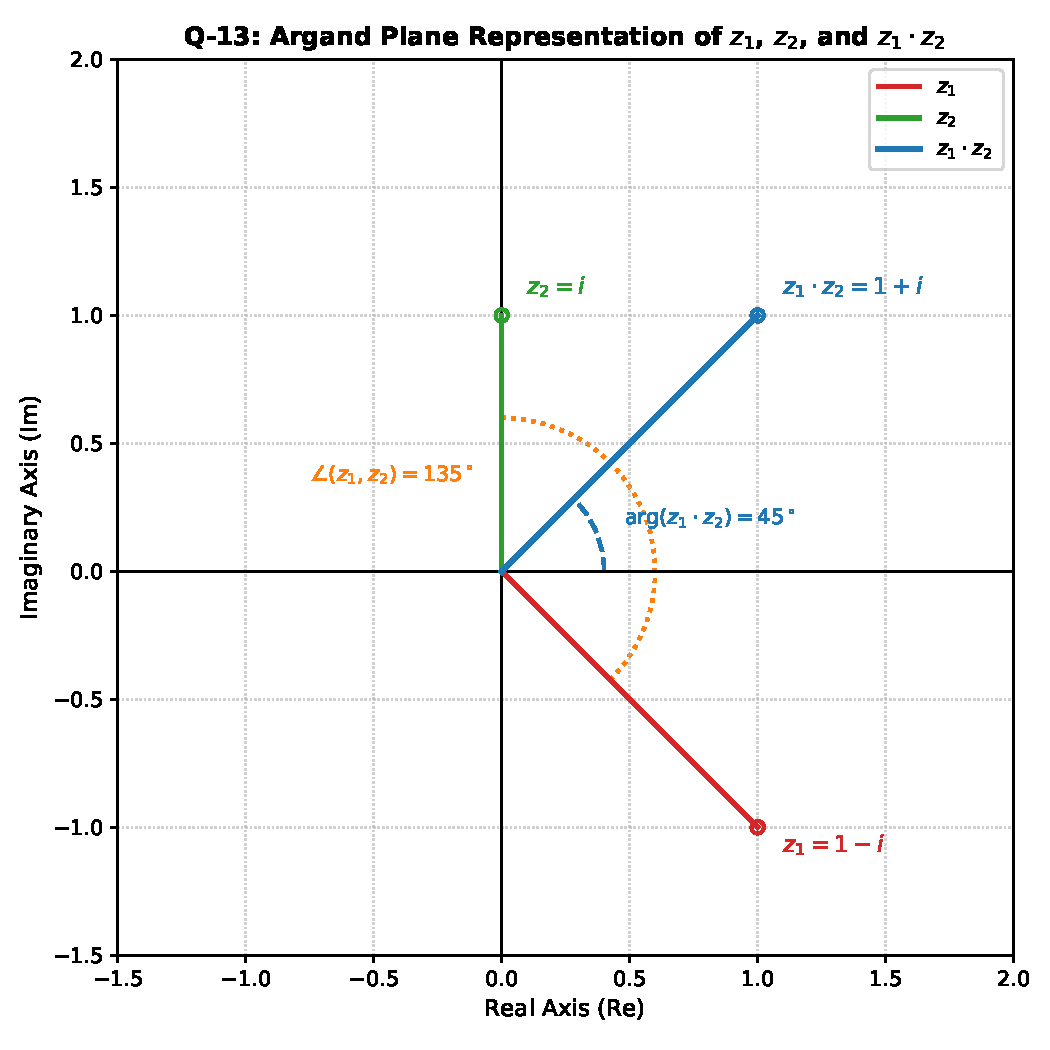
\includegraphics[width=1\linewidth]{figs/q13/Argument-Complex.pdf}
    \caption{Complex-plane representation of $z_1z_2$}
    \label{fig:ch25_q13}
\end{figure}

The code to verify this is:
\begin{lstlisting}[frame=single, basicstyle=\rmfamily, escapeinside={(*@}{@*)}]
(*@\makebox[\dimexpr\linewidth-2\fboxsep-2\fboxrule\relax][c]{codes/q13/main.py}@*)
\end{lstlisting}

% ----------------------------------------------------------- GATE Q14
\problem A box contains 3 identical green balls and 7 identical blue balls. Two balls are randomly drawn without replacement from the box. The probability of drawing 1 green and 1 blue ball is \hfill (GATE~CH~2025)
\begin{enumerate}[itemsep=0pt]
    \begin{multicols}{2}
        \item $\dfrac{{}^3P_1\times{}^7P_1}{{}^{10}P_2}$
        \item $\dfrac{{}^{10}P_3\times{}^{10}P_7}{{}^{10}P_2}$
        \item $\dfrac{{}^{10}C_3\times{}^{10}C_7}{{}^{10}C_2}$
        \item $\dfrac{{}^3C_1\times{}^7C_1}{{}^{10}C_2}$
    \end{multicols}
\end{enumerate}

\solution There are 3+7=10 balls in total. We need one green ball and one blue ball.

Using the combination formula in \eqref{eq:combination_formula}, the number of favourable selections is
\begin{align}
{}^3C_1\,{}^7C_1.
\end{align}
The total number of ways of selecting two balls from ten balls is
\begin{align}
{}^{10}C_2.
\end{align}
Therefore,
\begin{align}
P(1\text{ green},1\text{ blue})
&=\frac{{}^3C_1\,{}^7C_1}{{}^{10}C_2}\\
&=\frac{3\times7}{\frac{10\times9}{2}}\\
&=\frac{21}{45}\\
&=\frac{7}{15}.
\end{align}
The code and data to verify this are:
\begin{lstlisting}[frame=single, basicstyle=\rmfamily, escapeinside={(*@}{@*)}]
(*@\makebox[\dimexpr\linewidth-2\fboxsep-2\fboxrule\relax][c]{codes/q14/main.c}@*)
\end{lstlisting}

\begin{lstlisting}[frame=single, basicstyle=\rmfamily, escapeinside={(*@}{@*)}]
(*@\makebox[\dimexpr\linewidth-2\fboxsep-2\fboxrule\relax][c]{codes/q14/main.dat}@*)
\end{lstlisting}

% ----------------------------------------------------------- GATE Q35
\problem The residence time distribution function $E(t)$ for a reactor is given by
\begin{align}
E(t)=\begin{cases}
1-2t, & t\leq0.5\text{ min},\\
0, & t>0.5\text{ min}.
\end{cases}
\end{align}
The mean residence time (in min) is \underline{\hspace{2cm}} (rounded off to two decimal places). \hfill (GATE~CH~2025)

\solution Using the mean residence-time relation in \eqref{eq:mean_rtd_ratio},
\begin{align}
\bar{t}=\frac{\displaystyle\int_0^\infty tE(t)\,dt}{\displaystyle\int_0^\infty E(t)\,dt}.
\end{align}
Since $E(t)=0$ for $t>0.5$,
\begin{align}
\bar{t}=\frac{\displaystyle\int_0^{0.5}t(1-2t)\,dt}{\displaystyle\int_0^{0.5}(1-2t)\,dt}.
\end{align}
For the numerator,
\begin{align}
\int_0^{0.5}t(1-2t)\,dt
&=\int_0^{0.5}(t-2t^2)\,dt\\
&=\left[\frac{t^2}{2}-\frac{2t^3}{3}\right]_0^{0.5}\\
&=\frac18-\frac1{12}\\
&=\frac1{24}.
\end{align}
For the denominator,
\begin{align}
\int_0^{0.5}(1-2t)\,dt
&=\left[t-t^2\right]_0^{0.5}\\
&=\frac12-\frac14\\
&=\frac14.
\end{align}
Hence,
\begin{align}
\bar{t}&=\frac{1/24}{1/4}=\frac16=0.1667\text{ min}\\
&\approx0.17\text{ min}.
\end{align}

\begin{figure}[H]
    \centering
    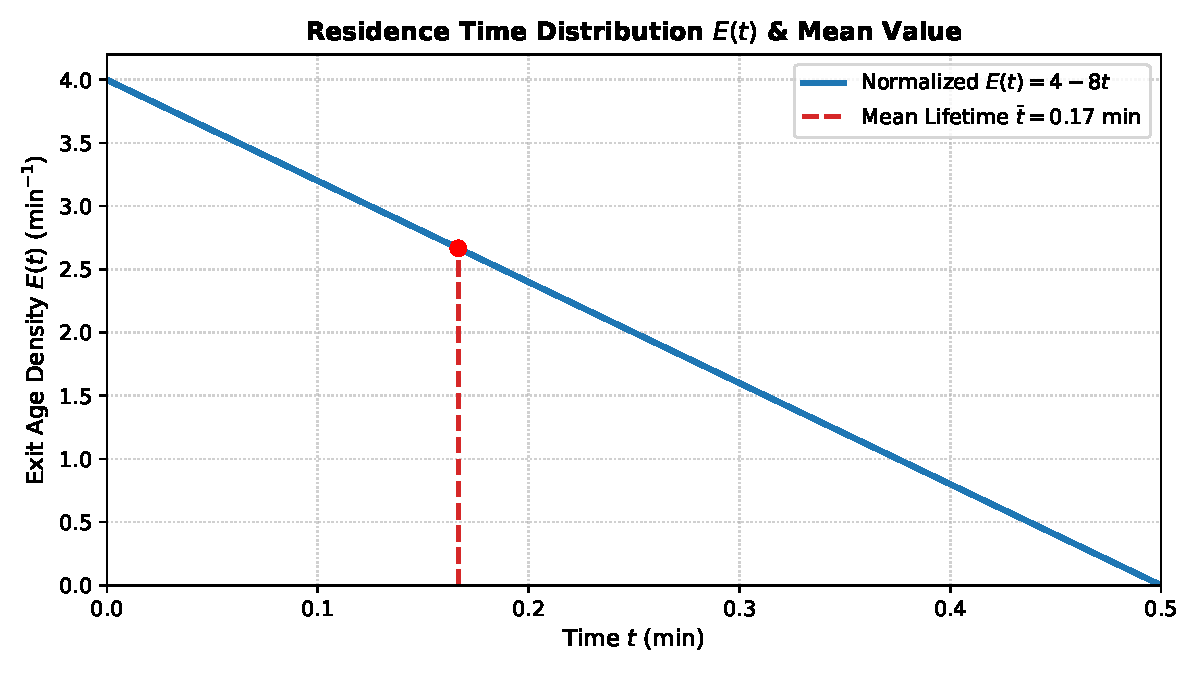
\includegraphics[width=1\linewidth]{figs/q35/RTD-Plot.pdf}
    \caption{Residence time distribution $E(t)$ for the given reactor}
    \label{fig:ch25_q35}
\end{figure}
The code to verify this is:
\begin{lstlisting}[frame=single, basicstyle=\rmfamily, escapeinside={(*@}{@*)}]
(*@\makebox[\dimexpr\linewidth-2\fboxsep-2\fboxrule\relax][c]{codes/q35/main.py}@*)
\end{lstlisting}

% ----------------------------------------------------------- GATE Q36
\problem Consider a Cartesian coordinate system in the $x-y$ plane, where $x,y\in[0,1]$. Let the vector be
\begin{align}
\vec{v}=ax\hat{i}-by\hat{j}.
\end{align}
Which one of the following conditions is required for the divergence of $\vec{v}$ to be zero? \hfill (GATE~CH~2025)
\begin{enumerate}[itemsep=0pt]
    \begin{multicols}{2}
        \item $a-b=0$
        \item $a<b$
        \item $a>b$
        \item $a+b=0$
    \end{multicols}
\end{enumerate}

\solution For a vector field, the Jacobian matrix is given by \eqref{eq:jacobian}, and the divergence is related to its trace by \eqref{eq:divergence_trace}.

For
\begin{align}
\vec{v}=v_x\hat{i}+v_y\hat{j},
\end{align}
the Jacobian is
\begin{align}
J_{\vec{v}}=
\myvec{
\dfrac{\partial v_x}{\partial x} & \dfrac{\partial v_x}{\partial y}\\
\dfrac{\partial v_y}{\partial x} & \dfrac{\partial v_y}{\partial y}
}.
\end{align}
The divergence is the trace:
\begin{align}
\nabla\cdot\vec{v}
&=\operatorname{tr}(J_{\vec{v}})\\
&=\frac{\partial v_x}{\partial x}+\frac{\partial v_y}{\partial y}.
\end{align}
Here,
\begin{align}
v_x=ax,\qquad v_y=-by.
\end{align}
Therefore,
\begin{align}
\frac{\partial v_x}{\partial x}=a,
\qquad
\frac{\partial v_y}{\partial y}=-b.
\end{align}
Thus,
\begin{align}
\nabla\cdot\vec{v}=a-b.
\end{align}
For zero divergence,
\begin{align}
a-b=0.
\end{align}

The code to verify this is:
\begin{lstlisting}[frame=single, basicstyle=\rmfamily, escapeinside={(*@}{@*)}]
(*@\makebox[\dimexpr\linewidth-2\fboxsep-2\fboxrule\relax][c]{codes/q36/main.py}@*)
\end{lstlisting}

% ----------------------------------------------------------- GATE Q37
\problem Let $X$ be a continuous random variable with probability density function
\begin{align}
p(x)=\begin{cases}
\dfrac{1}{a}, & x\in(0,a),\\
0, & \text{otherwise},
\end{cases}
\end{align}
where $a$ is a positive constant. Let $f(x)=x^2$. The expected value of $f(X)$ is \hfill (GATE~CH~2025)
\begin{enumerate}[itemsep=0pt]
    \begin{multicols}{2}
        \item $\dfrac{a^2}{3}$
        \item $\dfrac{a^3}{3}$
        \item $\dfrac{2a^2}{3}$
        \item $\dfrac{2a^3}{3}$
    \end{multicols}
\end{enumerate}

\solution The given function and probability density are
\begin{align}
f(x)&=x^2,\\
p(x)&=\frac1a,\qquad 0<x<a.
\end{align}
The expected value of a function of a continuous random variable is obtained from \eqref{eq:expectation_continuous}, which is the continuous form of taking a weighted average over all possible outcomes:
\begin{align}
E[f(X)]=\int_{-\infty}^{\infty}f(x)p(x)\,dx.
\end{align}
Since the density is non-zero only from $0$ to $a$,
\begin{align}
E[x^2]
&=\int_0^a x^2\frac1a\,dx\\
&=\frac1a\left[\frac{x^3}{3}\right]_0^a\\
&=\frac1a\frac{a^3}{3}\\
&=\frac{a^2}{3}.
\end{align}

The expected value represents the average output obtained when the possible outcomes are weighted according to their probabilities.


\begin{figure}[H]
    \centering
    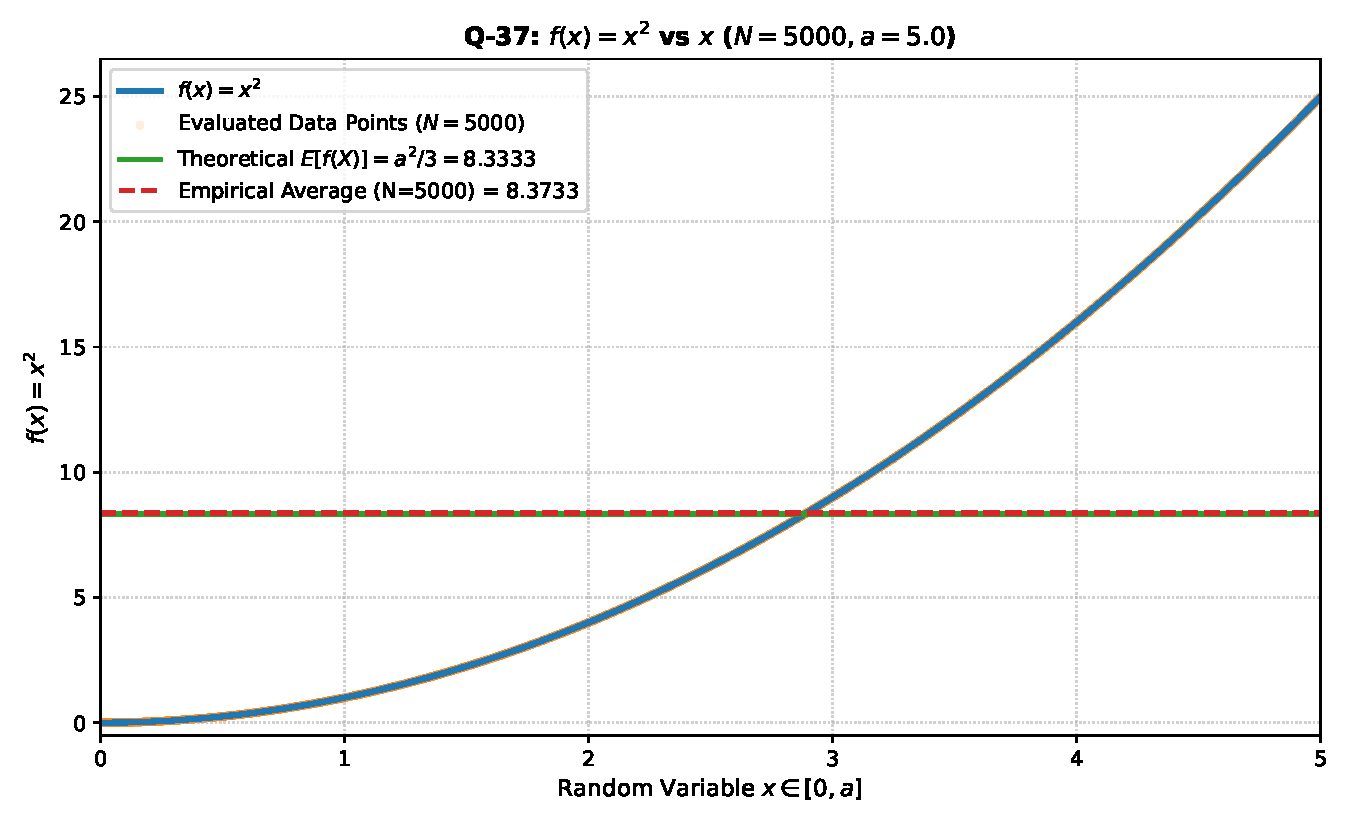
\includegraphics[width=1\linewidth]{figs/q37/Expected-Value.pdf}
    \caption{Uniform probability density over the interval $(0,a)$}
    \label{fig:ch25_q37}
\end{figure}
The codes and data to verify this are:
\begin{lstlisting}[frame=single, basicstyle=\rmfamily, escapeinside={(*@}{@*)}]
(*@\makebox[\dimexpr\linewidth-2\fboxsep-2\fboxrule\relax][c]{codes/q37/main.dat}@*)
\end{lstlisting}

\begin{lstlisting}[frame=single, basicstyle=\rmfamily, escapeinside={(*@}{@*)}]
(*@\makebox[\dimexpr\linewidth-2\fboxsep-2\fboxrule\relax][c]{codes/q37/main.py}@*)
\end{lstlisting}

\begin{lstlisting}[frame=single, basicstyle=\rmfamily, escapeinside={(*@}{@*)}]
(*@\makebox[\dimexpr\linewidth-2\fboxsep-2\fboxrule\relax][c]{codes/q37/main.c}@*)
\end{lstlisting}

% ----------------------------------------------------------- GATE Q44
\problem The differential equation
\begin{align}
\frac{dy}{dx}+\frac{y}{x}=0
\end{align}
has which of the following correct solution(s)? \hfill (GATE~CH~2025)
\begin{enumerate}[itemsep=0pt]
    \begin{multicols}{2}
        \item $y=x+c$
        \item $y=\dfrac{c}{x}$
        \item $y=-x+c$
        \item $y=0$
    \end{multicols}
\end{enumerate}

\solution
Rearranging the differential equation,
\begin{align}
\frac{dy}{dx}=-\frac{y}{x}.
\end{align}

For numerical plotting, the trapezoidal method approximates the solution using the average slope over a step. For
$f(x,y)=-y/x$, the update is
\begin{align}
y_{n+1}
&=y_n+\frac{h}{2}
\left[
-\frac{y_n}{x_n}
-\frac{y_{n+1}}{x_{n+1}}
\right].
\end{align}

The analytical solution is obtained by separation of variables:
\begin{align}
\frac{1}{y}\,dy=-\frac{1}{x}\,dx.
\end{align}

Integrating,
\begin{align}
\ln|y|&=-\ln|x|+C,\\
\ln|xy|&=C,\\
y&=\frac{C}{x}.
\end{align}

For $C=0$,
\begin{align}
y=0.
\end{align}

So as we solve for y, we end up with either $y = 0$ or $y = \frac{C}{x}$. \\

The trapezoidal method can then be used to generate numerical points for plotting the solution family.

\begin{figure}[H]
    \centering
    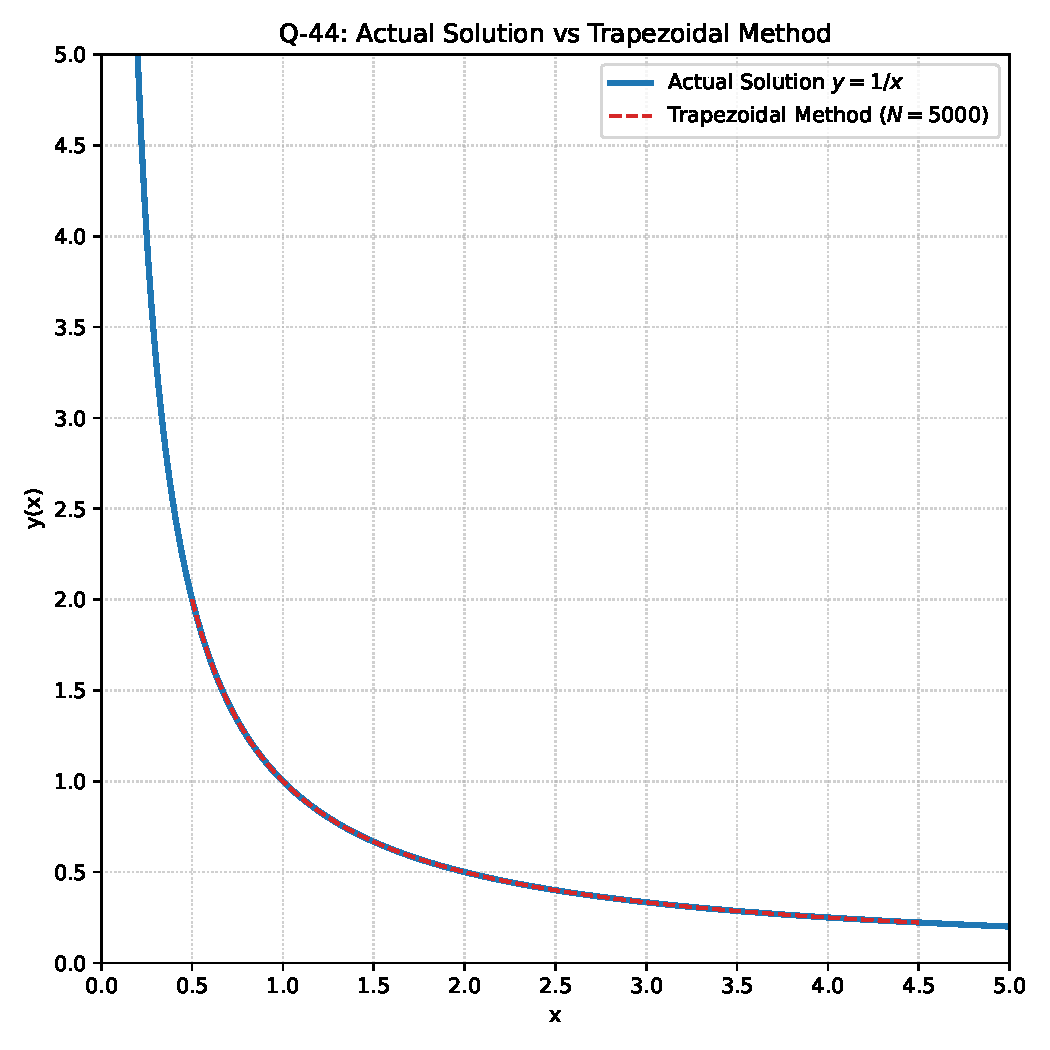
\includegraphics[width=1\linewidth]{figs/q44/Diff-Eqn.pdf}
    \caption{Solution family $y=C/x$ for the given differential equation}
    \label{fig:ch25_q44}
\end{figure}
The code to verify this is:
\begin{lstlisting}[frame=single, basicstyle=\rmfamily, escapeinside={(*@}{@*)}]
(*@\makebox[\dimexpr\linewidth-2\fboxsep-2\fboxrule\relax][c]{codes/q44/main.py}@*)
\end{lstlisting}

% ----------------------------------------------------------- GATE Q45
\problem Consider the matrix
\begin{align}
\vec{A}=\myvec{2&3\\1&2}.
\end{align}
One of its eigenvalues is $0.27$. The other eigenvalue, rounded off to two decimal places, is \underline{\hspace{2cm}}. \hfill (GATE~CH~2025)

\solution For an eigenvalue $\lambda$ and its corresponding eigenvector $\vec{x}$,
\begin{align}
\vec{A}\vec{x}=\lambda\vec{x},\qquad \vec{x}\ne\vec{0}.
\end{align}
The eigenvalues are obtained from the characteristic equation
\begin{align}
\left| \vec{A}-\lambda\vec{I} \right|=0.
\end{align}
For the given matrix,
\begin{align}
\left| 
\begin{matrix} 
	2-\lambda & 3 \\ 
	1 & 2-\lambda 
\end{matrix} 
\right| =0.
\end{align}
Therefore,
\begin{align}
(2-\lambda)^2-3&=0\\
\lambda^2-4\lambda+1&=0.
\end{align}
Solving the quadratic equation,
\begin{align}
\lambda&=\frac{4\pm\sqrt{16-4}}{2}\\
&=2\pm\sqrt{3}.
\end{align}
Thus,
\begin{align}
\lambda_1&=2-\sqrt{3}\approx0.27,\\
\lambda_2&=2+\sqrt{3}\approx3.73.
\end{align}

For completeness, the corresponding eigenvectors can be obtained from $(\vec{A}-\lambda\vec{I})\vec{x}=0$. For $\lambda_1=2-\sqrt{3}$,
\begin{align}
\sqrt{3}x+3y&=0,
\end{align}
so one eigenvector is
\begin{align}
\vec{x}_1=\myvec{\sqrt{3}\\-1}.
\end{align}
For $\lambda_2=2+\sqrt{3}$,
\begin{align}
-\sqrt{3}x+3y&=0,
\end{align}
so one eigenvector is
\begin{align}
\vec{x}_2=\myvec{\sqrt{3}\\1}.
\end{align}

From the trace relation in \eqref{eq:eigen_trace}, the sum of the eigenvalues is
\begin{align}
\lambda_1+\lambda_2&=(2-\sqrt{3})+(2+\sqrt{3})\\
&=4.
\end{align}
The trace of the matrix is
\begin{align}
\operatorname{tr}(\vec{A})=2+2=4.
\end{align}
Hence,
\begin{align}
\boxed{\lambda_1+\lambda_2=\operatorname{tr}(\vec{A})}.
\end{align}
Using the given value $\lambda_1=0.27$ and the trace,
\begin{align}
\lambda_2&=4-0.27\\
&=3.73.
\end{align}
The code to verify this is:
\begin{lstlisting}[frame=single, basicstyle=\rmfamily, escapeinside={(*@}{@*)}]
(*@\makebox[\dimexpr\linewidth-2\fboxsep-2\fboxrule\relax][c]{codes/q45/main.py}@*)
\end{lstlisting}

% ----------------------------------------------------------- GATE Q46
\problem The Newton-Raphson method is used to obtain the root of
\begin{align}
f(x)=x^2-x-1=0
\end{align}
with the initial guess $x_{0}=1$. The value of the second iterate $x_{2}$, rounded off to two decimal places, is \underline{\hspace{2cm}}. \hfill (GATE~CH~2025)

\solution Newton-Raphson improves an initial guess by using the tangent to the function at the current point. Repeating the iteration moves the approximation towards the root.

The Newton-Raphson formula is given by \eqref{eq:newton_raphson}:
\begin{align}
x_{(n+1)}=x_{n}-\frac{f(x_{n})}{f'(x_{n})}.
\end{align}
Here,
\begin{align}
f(x)&=x^2-x-1,\\
f'(x)&=2x-1.
\end{align}
Given
\begin{align}
x_{0}=1.
\end{align}
For the first iteration,
\begin{align}
f(1)&=-1,\\
f'(1)&=1,
\end{align}
and hence
\begin{align}
x_{1}&=1-\frac{-1}{1}=2.
\end{align}
For the second iteration,
\begin{align}
f(2)&=4-2-1=1,\\
f'(2)&=4-1=3.
\end{align}
Therefore,
\begin{align}
x_{2}&=2-\frac{1}{3}\\
&=\frac53\\
&=1.6667\ldots
\end{align}
Thus, rounded off to two decimal places, $x_{2}=1.67$.

\begin{figure}[H]
    \centering
    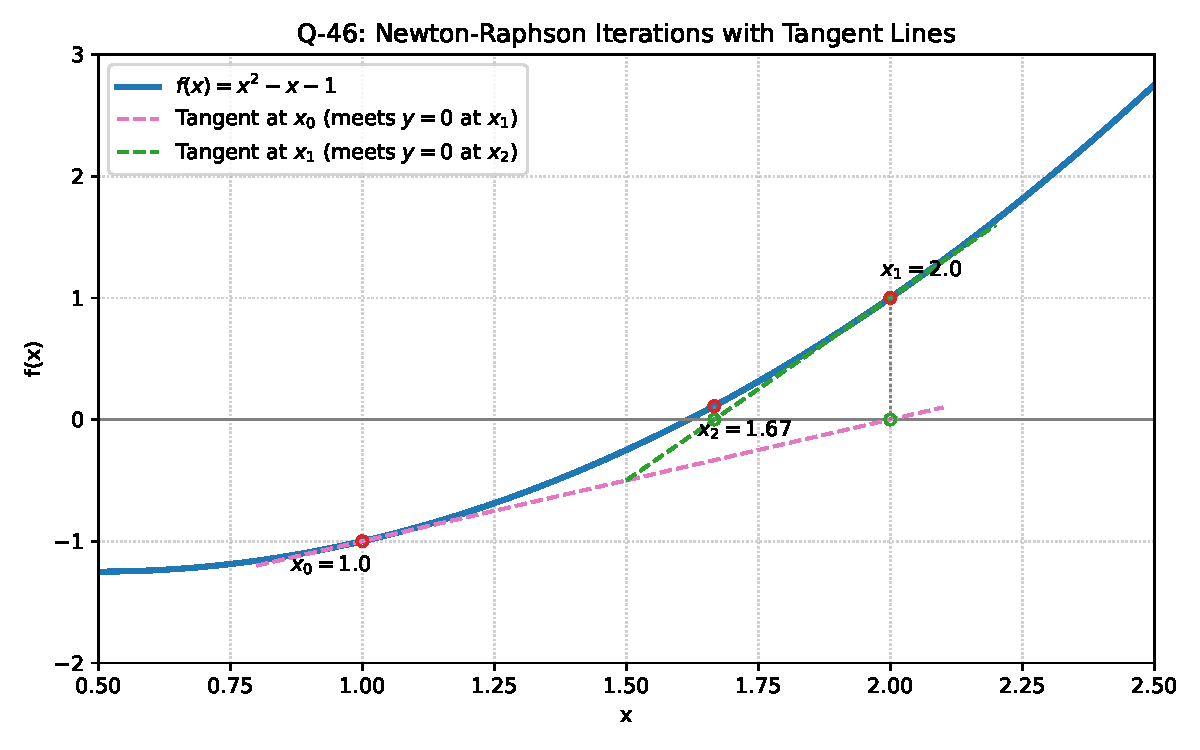
\includegraphics[width=1\linewidth]{figs/q46/Newton-Raphson.pdf}
    \caption{Newton-Raphson iteration for $f(x)=x^2-x-1$}
    \label{fig:ch25_q46}
\end{figure}
The code to verify this is:
\begin{lstlisting}[frame=single, basicstyle=\rmfamily, escapeinside={(*@}{@*)}]
(*@\makebox[\dimexpr\linewidth-2\fboxsep-2\fboxrule\relax][c]{codes/q46/main.py}@*)
\end{lstlisting}

% ----------------------------------------------------------- GATE Q60
\problem The transfer function of a process is
\begin{align}
G_p(s)=\frac{2e^{-s}}{(5s+1)^2}.
\end{align}
The process is fitted to a first-order plus dead-time (FOPDT) model using the maximum slope method. If $\tau_m$ and $\theta_m$ are the fitted time constant and dead time, respectively, then $\tau_m/\theta_m$, rounded off to two decimal places, is \underline{\hspace{2cm}}. \hfill (GATE~CH~2025)

The unit-step response and its derivatives for $1/(\tau s+1)^2$ are
\begin{align}
y(t)&=1-\left(1+\frac{t}{\tau}\right)e^{-t/\tau},\\
\frac{dy}{dt}&=\frac{t}{\tau^2}e^{-t/\tau},\\
\frac{d^2y}{dt^2}&=\frac{1}{\tau^2}\left(1-\frac{t}{\tau}\right)e^{-t/\tau}.
\end{align}

\solution From the time-delay relation, the factor $e^{-s}$ represents a pure time delay of $1$ min. Thus the dynamic response of the second-order part is shifted by $1$ min.

For the dynamic part,
\begin{align}
G_0(s)=\frac{2}{(5s+1)^2},
\end{align}
so
\begin{align}
K=2,\qquad \tau=5\text{ min},\qquad \theta=1\text{ min}.
\end{align}
For the normalized second-order response, the maximum slope occurs at the inflection point, where
\begin{align}
\frac{d^2y}{dt^2}=0.
\end{align}
Hence,
\begin{align}
1-\frac{t}{\tau}=0\implies t=\tau=5\text{ min}.
\end{align}
Including the dead time,
\begin{align}
t_{\mathrm{inflection}}=1+5=6\text{ min}.
\end{align}
At this point, the output is
\begin{align}
y_{\mathrm{inflection}}
&=2\left[1-\left(1+\frac55\right)e^{-1}\right]\\
&=2\left(1-\frac2e\right).
\end{align}
The maximum slope is
\begin{align}
R
&=2\left[\frac{t}{\tau^2}e^{-t/\tau}\right]_{t=5}\\
&=\frac{2}{5e}.
\end{align}
Using the maximum-slope relations in \eqref{eq:maximum_slope} and \eqref{eq:fopdt_time_constant}, the fitted time constant is
\begin{align}
\tau_m&=\frac{K\Delta u}{R}\\
&=\frac{2\times1}{2/(5e)}\\
&=5e.
\end{align}
Using the dead-time tangent relation in \eqref{eq:dead_time_tangent}, the tangent at the inflection point intersects the time axis at
\begin{align}
\theta_m
&=t_{\mathrm{inflection}}-\frac{y_{\mathrm{inflection}}}{R}\\
&=6-\frac{2(1-2/e)}{2/(5e)}\\
&=16-5e.
\end{align}
Therefore,
\begin{align}
\frac{\tau_m}{\theta_m}
&=\frac{5e}{16-5e}\\
&\approx5.64.
\end{align}

\begin{figure}[H]
    \centering
    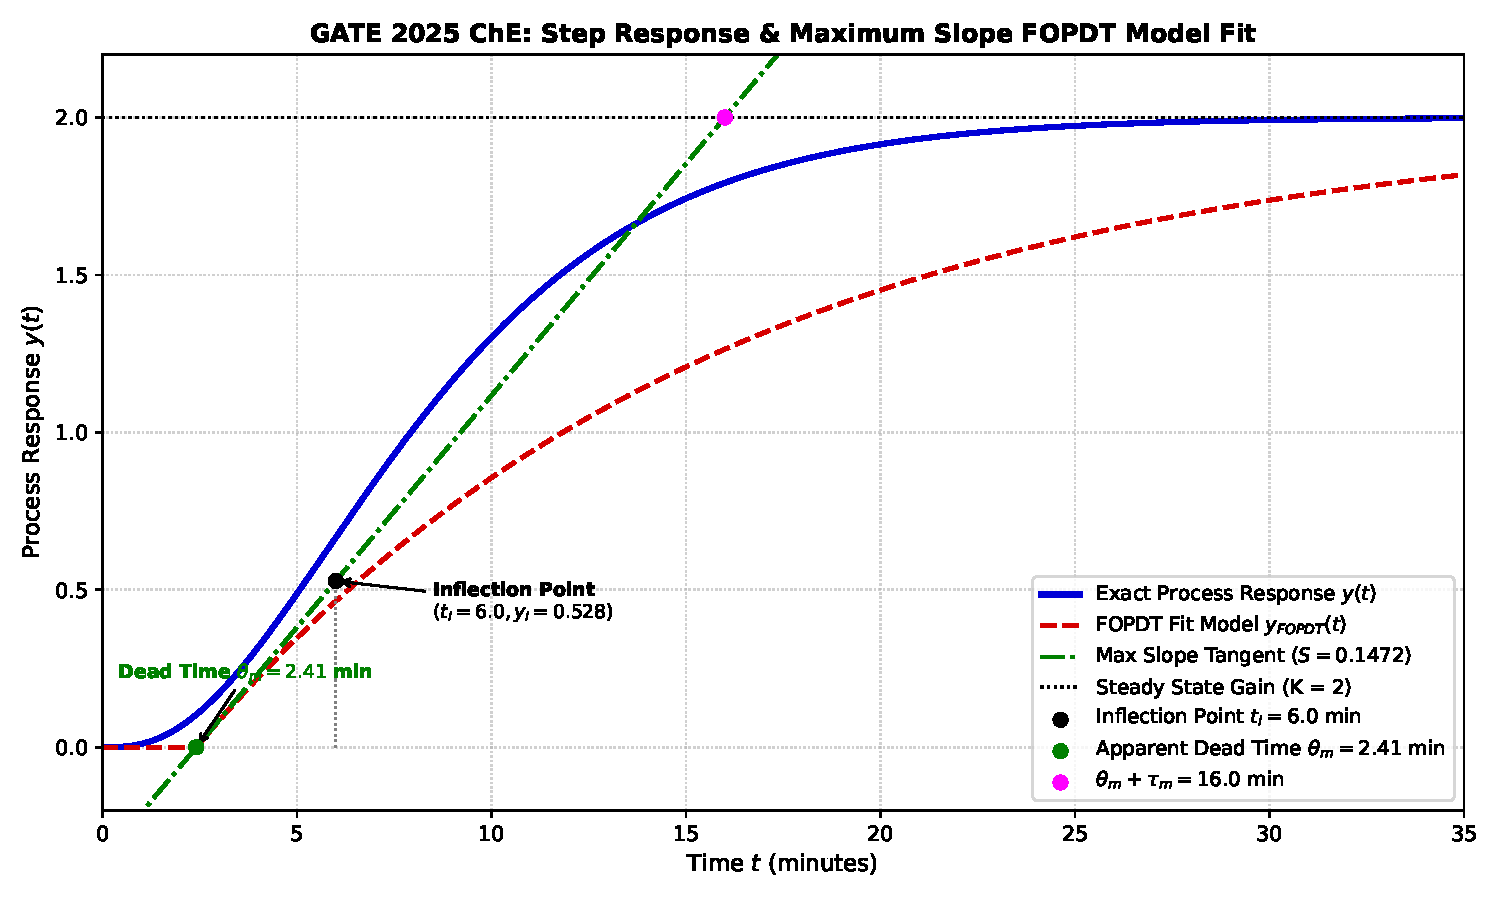
\includegraphics[width=1\linewidth]{figs/q60/FOPDT-Modelling.pdf}
    \caption{Maximum-slope FOPDT approximation of the given process response}
    \label{fig:ch25_q60}
\end{figure}
The code to verify this is:
\begin{lstlisting}[frame=single, basicstyle=\rmfamily, escapeinside={(*@}{@*)}]
(*@\makebox[\dimexpr\linewidth-2\fboxsep-2\fboxrule\relax][c]{codes/q60/main.py}@*)
\end{lstlisting}

% ----------------------------------------------------------- GATE Q62
\problem The block diagram of a series cascade control system (with time in minutes) is shown in the figure. For $\tau_I=8$ min and $K_c^s=1$, the maximum value of $K_c^m$, below which the cascade control system is stable, is \underline{\hspace{2cm}} (rounded off to the nearest integer). \hfill (GATE~CH~2025)

\begin{figure}[H]
    \centering
    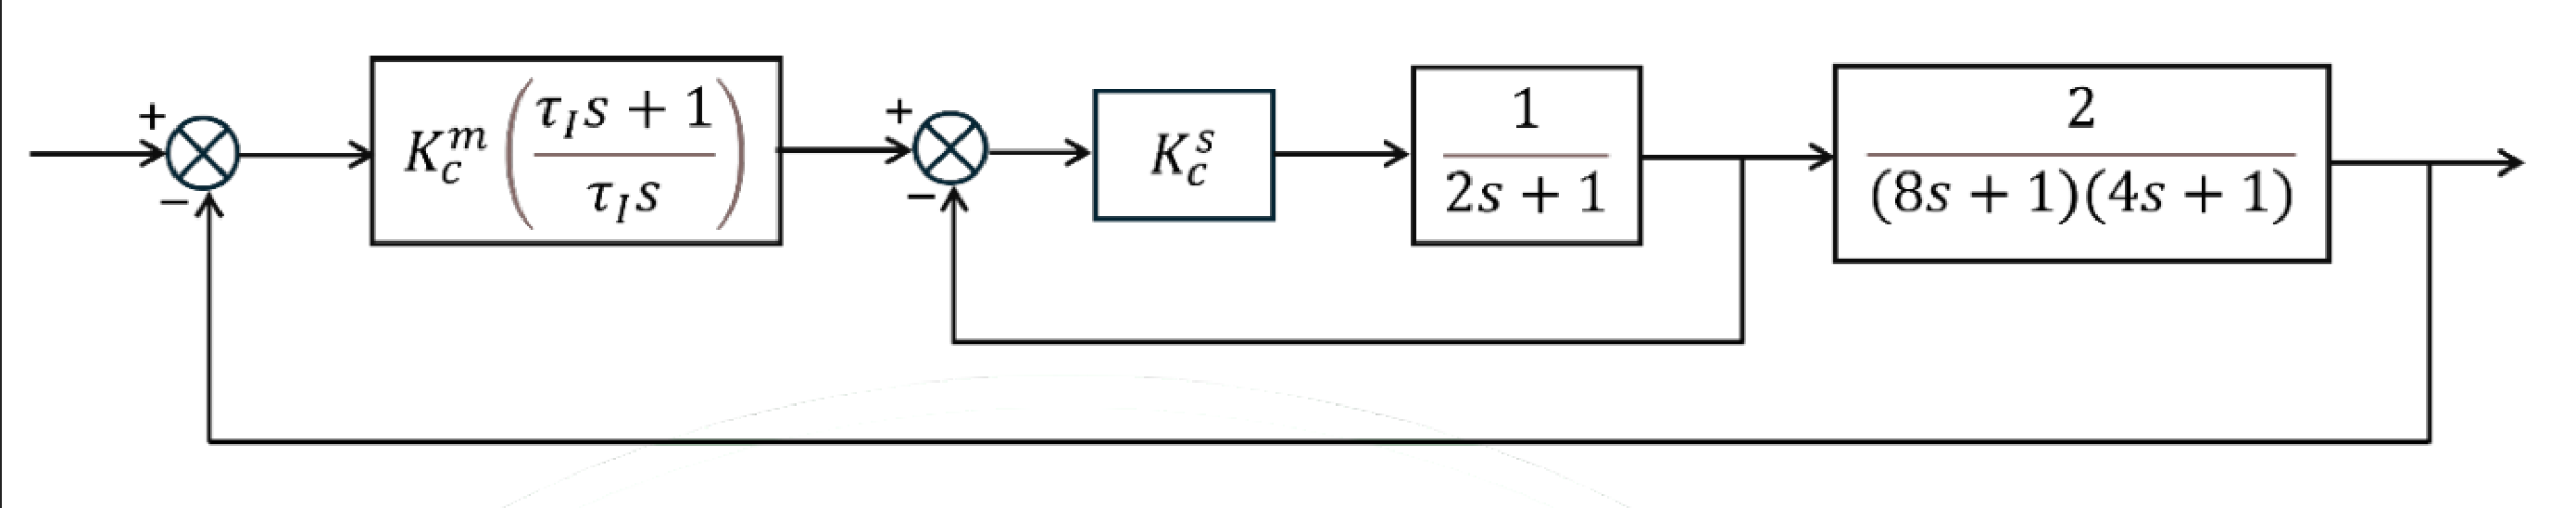
\includegraphics[width=1\linewidth]{figs/q62/Q62-Problem.pdf}
    \caption{Series cascade control system given in GATE CH 2025 Q62}
    \label{fig:ch25_q62_problem}
\end{figure}

\solution The inner process is
\begin{align}
G_1(s)=\frac{1}{2s+1},
\end{align}
and the inner controller gain is $K_c^s=1$. Therefore, the closed-loop inner transfer function is
\begin{align}
G_{\mathrm{inner}}(s)
&=\frac{K_c^sG_1(s)}{1+K_c^sG_1(s)}\\
&=\frac{1/(2s+1)}{1+1/(2s+1)}\\
&=\frac{1}{2(s+1)}.
\end{align}
The outer process is
\begin{align}
G_2(s)=\frac{2}{(8s+1)(4s+1)}.
\end{align}
Hence the equivalent process for the outer loop is
\begin{align}
G_{\mathrm{eq}}(s)
&=G_{\mathrm{inner}}(s)G_2(s)\\
&=\frac{1}{(s+1)(8s+1)(4s+1)}.
\end{align}
The outer controller is
\begin{align}
G_c(s)=K_c^m\frac{\tau_Is+1}{\tau_Is}.
\end{align}
Since $\tau_I=8$ min,
\begin{align}
G_c(s)=K_c^m\frac{8s+1}{8s}.
\end{align}
Therefore, the open-loop transfer function of the outer loop is
\begin{align}
G_c(s)G_{\mathrm{eq}}(s)
&=K_c^m\frac{8s+1}{8s(s+1)(8s+1)(4s+1)}\\
&=\frac{K_c^m}{8s(s+1)(4s+1)}.
\end{align}
For unity negative feedback, using \eqref{eq:unity_closed_loop}, the characteristic equation is
\begin{align}
1+\frac{K_c^m}{8s(s+1)(4s+1)}=0,
\end{align}
which gives
\begin{align}
8s(s+1)(4s+1)+K_c^m&=0\\
32s^3+40s^2+8s+K_c^m&=0.
\end{align}
Using the Routh-Hurwitz relations in \eqref{eq:routh_array}, the Routh array is
\begin{align}
\myvec{
32 & 8\\
40 & K_c^m\\
\dfrac{40(8)-32K_c^m}{40} & 0\\
K_c^m &
}.
\end{align}
For stability, every element in the first column must be positive. Thus,
\begin{align}
8-0.8K_c^m&>0,\\
K_c^m&>0.
\end{align}
Therefore,
\begin{align}
0<K_c^m<10.
\end{align}
Hence the maximum value of $k_c^m$ below which the system is stable, rounded to the nearest integer, is 10.

\begin{figure}[H]
    \centering
    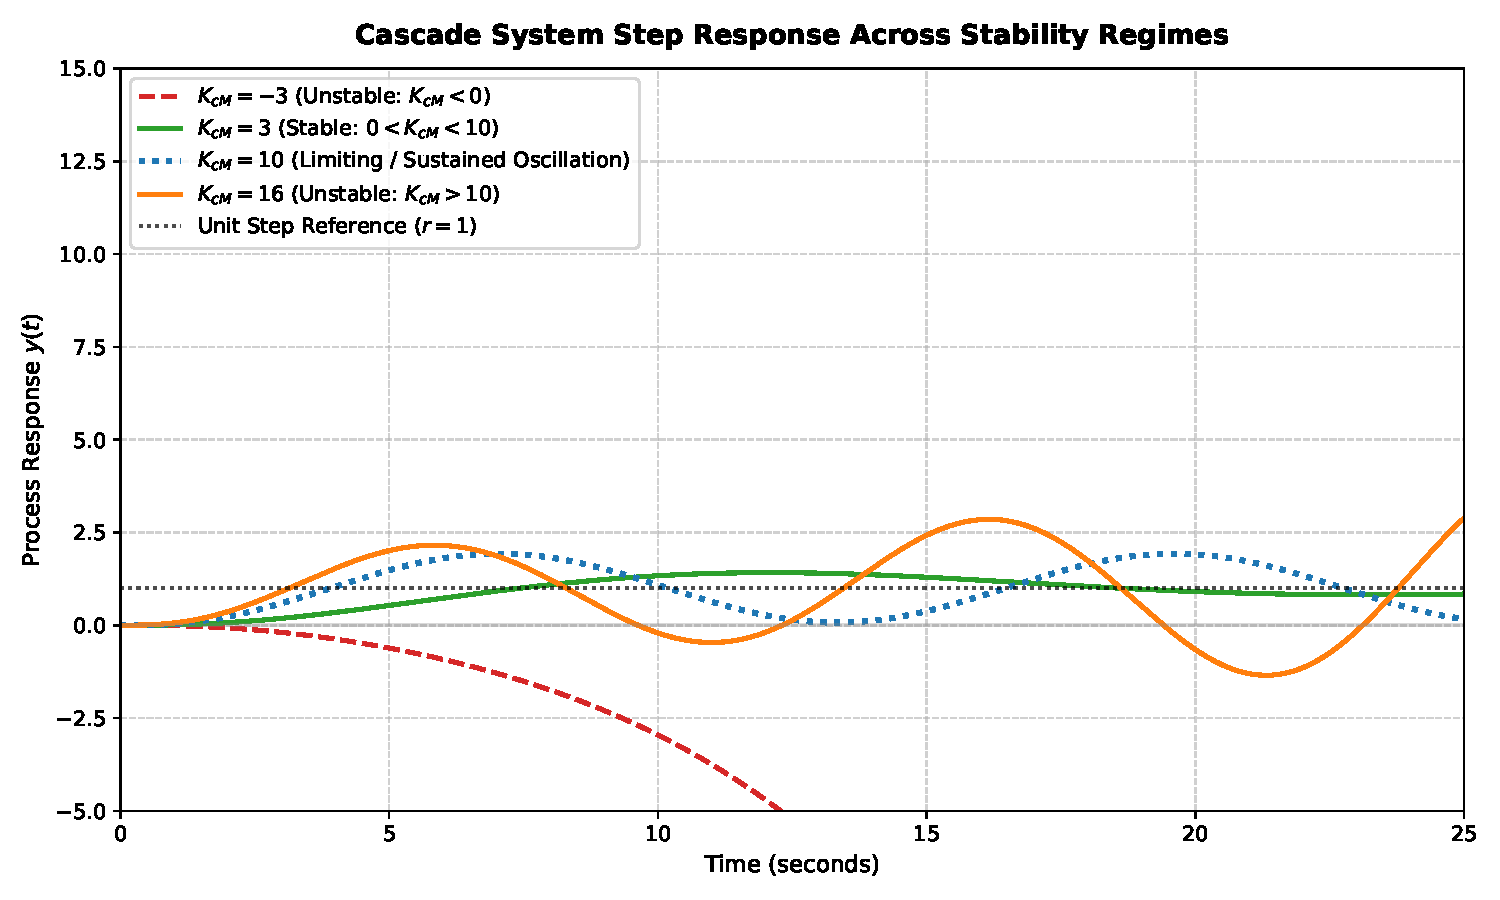
\includegraphics[width=1\linewidth]{figs/q62/Response-Plot.pdf}
    \caption{Cascade-loop reduction and Routh-Hurwitz stability calculation for Q62}
    \label{fig:ch25_q62_solution}
\end{figure}
The code to verify this is:
\begin{lstlisting}[frame=single, basicstyle=\rmfamily, escapeinside={(*@}{@*)}]
(*@\makebox[\dimexpr\linewidth-2\fboxsep-2\fboxrule\relax][c]{codes/q62/main.py}@*)
\end{lstlisting}

\end{enumerate}
